\documentclass[12pt]{article}

\usepackage{hcmus-report-template}

\usepackage{graphicx}
\usepackage{float}
\usepackage{placeins}
\usepackage{tabularx}
\usepackage{booktabs}
\usepackage{enumitem}
\usepackage{tikz}
\usetikzlibrary{arrows.meta,positioning,fit,calc,shapes.geometric}

% Disable indentation on new paragraphs
\setlength{\parindent}{0pt}

% Line spacing 1.5
\renewcommand{\baselinestretch}{1.5}

% Graphic paths
\graphicspath{{img/}{../slide/images/}{../screenshot/}}

% Times New Roman equivalent
\usepackage{mathptmx}

% Define course name, report name and report title.
\newcommand{\coursename}{Nhập môn Dữ liệu lớn}
\newcommand{\reportname}{A Triple of Vector Stores: Qdrant, Weaviate, and Milvus}
\newcommand{\reporttitle}{BÁO CÁO SEMINAR CUỐI KÌ}

\newcommand{\studentname}{Lê Xuân Trí - 23120099 \\ Nguyễn Hồ Anh Tuấn - 23120185 \\ Trần Hữu Kim Thành - 23120166 \\ Trần Lê Trung Trực - 23120180}
\newcommand{\teachername}{Thầy Trần Huy Bân}

% Header
\lhead{\reporttitle}
\rhead{
Trường Đại học Khoa học Tự nhiên - ĐHQG HCM\\
\coursename
}

% TikZ styles for architecture diagrams
\tikzset{
  flowbox/.style={draw=black!50, fill=blue!5, rounded corners=2pt, align=center, minimum height=0.7cm, inner xsep=5pt, inner ysep=3pt, font=\small},
  flowarrow/.style={-{Stealth[length=2.2mm]}, thick, draw=black!70},
}

% ============ DOCUMENT ============
\begin{document}

\pagenumbering{roman}
\input{content/title}

\cleardoublepage
\setcounter{page}{2}
\pagestyle{empty} 

\tableofcontents

\cleardoublepage
\pagenumbering{arabic} 
\pagestyle{plain}

\setcounter{page}{1}

\section{Giới thiệu}
\label{sec:introduction}

Trong những năm gần đây, các mô hình ngôn ngữ lớn (Large Language Model -- LLM) như GPT, Gemini hay Qwen đã chứng minh khả năng sinh ngôn ngữ tự nhiên vượt trội. Tuy nhiên, LLM vẫn tồn tại ba giới hạn nghiêm trọng: (i)~kiến thức bị đóng băng tại thời điểm huấn luyện (\textit{knowledge cutoff}), (ii)~có thể sinh ra thông tin không chính xác một cách tự tin (\textit{hallucination}), và (iii)~không thể truy cập dữ liệu nội bộ của tổ chức~\cite{lewis2020rag}. Retrieval-Augmented Generation (RAG) là kiến trúc được đề xuất nhằm khắc phục cả ba giới hạn trên bằng cách bổ sung bước truy hồi ngữ cảnh (\textit{retrieval}) trước khi mô hình sinh câu trả lời.

\subsection{Vector Database và vai trò trong Big Data}

Trong pipeline RAG, tài liệu được chia thành các đoạn nhỏ (\textit{chunk}), mỗi đoạn được chuyển đổi thành vector embedding --- một mảng số thực nhiều chiều (thường 768--1536 chiều) biểu diễn ngữ nghĩa của đoạn văn bản. Các vector này được lưu trữ trong \textbf{Vector Database} --- một hệ quản trị cơ sở dữ liệu chuyên biệt cho việc lưu trữ và tìm kiếm vector nhiều chiều dựa trên độ tương đồng ngữ nghĩa.

Khác với cơ sở dữ liệu truyền thống (SQL, NoSQL) vốn tối ưu cho truy vấn chính xác (\texttt{WHERE}, \texttt{LIKE}), Vector Database giải quyết bài toán \textit{tìm kiếm theo ngữ nghĩa}: thay vì so khớp từ khóa, hệ thống tìm các chunk có ý nghĩa gần nhất với câu hỏi của người dùng. Hầu hết Vector Database hiện đại sử dụng thuật toán HNSW (Hierarchical Navigable Small World)~\cite{malkov2020hnsw} --- một thuật toán tìm kiếm láng giềng gần đúng (Approximate Nearest Neighbor -- ANN) dạng đồ thị đa tầng, cho phép truy vấn với độ trễ dưới 10\,ms trên tập dữ liệu hàng triệu vector~\cite{annbenchmarks}.

\subsection{Vai trò trong RAG, Semantic Search và AI Systems}

Pipeline RAG hoạt động theo hai pha. \textbf{Pha indexing}: tài liệu PDF được cắt thành chunk, embedding thành vector, và lưu vào Vector Database kèm metadata. \textbf{Pha answering}: câu hỏi của người dùng được embedding thành query vector, Vector Database tìm Top-K chunk gần nghĩa nhất, các chunk này được đưa vào prompt để LLM sinh câu trả lời có ngữ cảnh. Nếu tầng retrieval trả về context sai, LLM sẽ không có bằng chứng đáng tin cậy để trả lời chính xác dù bản thân mô hình rất mạnh.

\begin{figure}[H]
\centering
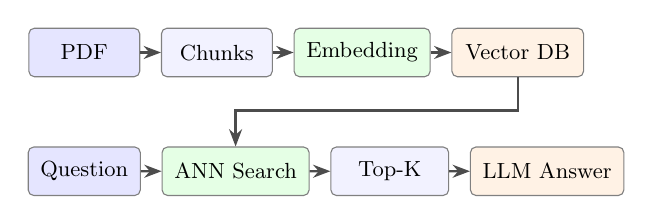
\begin{tikzpicture}[node distance=0.4cm and 0.3cm, scale=0.88, transform shape]
    \node[flowbox, fill=blue!10, minimum width=1.6cm] (pdf) {PDF};
    \node[flowbox, right=of pdf, minimum width=1.6cm] (chunks) {Chunks};
    \node[flowbox, right=of chunks, fill=green!10, minimum width=1.9cm] (embed) {Embedding};
    \node[flowbox, right=of embed, fill=orange!10, minimum width=1.9cm] (db) {Vector DB};
    \node[flowbox, below=1cm of pdf, fill=blue!10, minimum width=1.6cm] (q) {Question};
    \node[flowbox, right=of q, fill=green!10, minimum width=1.7cm] (search) {ANN Search};
    \node[flowbox, right=of search, minimum width=1.7cm] (ctx) {Top-K};
    \node[flowbox, right=of ctx, fill=orange!10, minimum width=1.8cm] (llm) {LLM Answer};
    \draw[flowarrow] (pdf) -- (chunks);
    \draw[flowarrow] (chunks) -- (embed);
    \draw[flowarrow] (embed) -- (db);
    \draw[flowarrow] (q) -- (search);
    \draw[flowarrow] (db.south) -- ++(0,-0.48) -| (search.north);
    \draw[flowarrow] (search) -- (ctx);
    \draw[flowarrow] (ctx) -- (llm);
\end{tikzpicture}
\caption{Pipeline RAG: pha indexing (trên) và pha answering (dưới).}
\label{fig:rag-pipeline}
\end{figure}

\subsection{Mục tiêu báo cáo}

Báo cáo này phân tích ba hệ quản trị Vector Database tiêu biểu --- \textbf{Qdrant}, \textbf{Weaviate} và \textbf{Milvus} --- từ góc nhìn kiến trúc, khả năng truy hồi, chi phí vận hành và tiêu chí lựa chọn cho production. Nhóm không chỉ tổng hợp lý thuyết mà còn xây dựng hệ thống benchmark full-stack để đánh giá bằng số liệu thực nghiệm.

\section{Tổng quan ba hệ quản trị Vector Database}
\label{sec:overview}

Qdrant, Weaviate và Milvus đều thuộc nhóm Vector Database: hệ quản trị dữ liệu được thiết kế để lưu trữ embedding, lập chỉ mục vector nhiều chiều và trả về các điểm dữ liệu gần nhất theo độ đo như cosine similarity, dot product hoặc Euclidean distance. Trong hệ thống Big Data hiện đại, lớp này thường đứng giữa data lake/document store và ứng dụng AI, đặc biệt trong Retrieval-Augmented Generation (RAG), semantic search, recommendation và duplicate detection. Điểm quan trọng là ba công cụ không tối ưu cho cùng một ràng buộc. Qdrant nhấn mạnh filtered vector search gọn nhẹ; Weaviate nhấn mạnh trải nghiệm xây dựng ứng dụng AI/hybrid RAG; Milvus nhấn mạnh scale phân tán và tách vai trò compute/storage.

\subsection{Qdrant}

Qdrant là Vector Database viết bằng \textbf{Rust}, ra đời năm 2021 bởi Qdrant Solutions GmbH. Triết lý thiết kế của Qdrant là \textit{performance-first}: giảm overhead runtime, giữ footprint gọn và tối ưu truy vấn có payload filter~\cite{qdrantdocs}. Trong mô hình dữ liệu của Qdrant, vector đi kèm payload dạng key-value; payload này có thể được lập chỉ mục để hỗ trợ các truy vấn như ``tìm đoạn văn gần nhất nhưng chỉ trong tài liệu của phòng ban X''. Vì vậy, Qdrant phù hợp với knowledge base hoặc RAG nhiều tenant, nơi mỗi truy vấn thường cần lọc theo quyền truy cập, loại tài liệu, domain hoặc thời gian.

\subsection{Weaviate}

Weaviate là Vector Database viết bằng \textbf{Go}, ra đời năm 2019 bởi Weaviate B.V. Điểm khác biệt cốt lõi là định hướng \textit{AI-native}: ngoài vector HNSW index, Weaviate còn duy trì inverted index cho keyword search và cung cấp module tích hợp vectorizer, reranker, generative model~\cite{weaviatedocs,weaviatemodules}. Weaviate vì thế không chỉ là một ANN engine, mà còn là một retrieval platform có schema object, hybrid score và GraphQL/REST API. Công cụ này phù hợp khi RAG cần kết hợp semantic search với keyword chính xác như tên riêng, mã sản phẩm, thuật ngữ chuyên ngành hoặc các truy vấn có phần ``literal match'' quan trọng.

\subsection{Milvus}

Milvus là Vector Database sử dụng \textbf{C++} cho lõi tính toán và \textbf{Go} cho các service điều phối, ra đời năm 2019 và là \textit{graduated project} của LF AI \& Data Foundation~\cite{wang2021milvus}. Milvus theo hướng \textit{distributed-first}: tách compute khỏi storage, chia vai trò thành Proxy, Coordinator, QueryNode, DataNode và IndexNode. Thay vì tối ưu cho trải nghiệm một container, Milvus tối ưu cho hệ thống enterprise có nhiều collection, corpus rất lớn, yêu cầu HA hoặc cần tận dụng nhiều loại index như IVF, HNSW, DiskANN/GPU thông qua Knowhere~\cite{milvusdocs}.

\subsection{Mức độ phổ biến trong cộng đồng}

GitHub stars, số lượng issue/PR, connector trong ecosystem AI và DB-Engines ranking chỉ nên xem là tín hiệu cộng đồng, không phải bằng chứng trực tiếp về chất lượng kỹ thuật. Tại thời điểm nhóm tổng hợp tài liệu cho seminar, Milvus có cộng đồng GitHub lớn nhất trong ba công cụ và xuất hiện sớm trong nhiều benchmark ANN/vector database; Qdrant tăng trưởng nhanh nhờ làn sóng RAG/AI agents và cách triển khai gọn; Weaviate nổi bật trong nhóm developer xây dựng hybrid RAG và ứng dụng có schema object rõ ràng~\cite{dbengines}. Vì vậy, trong bối cảnh Big Data, ba công cụ đều phổ biến nhưng phổ biến ở các phân khúc khác nhau: Milvus thiên về enterprise/scale, Qdrant thiên về production RAG gọn nhẹ, Weaviate thiên về developer-facing AI application.

\begin{table}[H]
\centering
\caption{Tổng quan thiết kế và phân khúc sử dụng của ba Vector Database.}
\label{tab:overview}
\resizebox{\textwidth}{!}{%
\begin{tabular}{lccc}
\toprule
\textbf{Tiêu chí} & \textbf{Qdrant} & \textbf{Weaviate} & \textbf{Milvus} \\
\midrule
Năm ra đời & 2021 & 2019 & 2019 \\
Ngôn ngữ core & Rust & Go & C++ \& Go \\
Trọng tâm thiết kế & Filtered vector search & Hybrid RAG platform & Enterprise vector scale \\
Đối tượng phù hợp & Team cần latency/footprint gọn & Ứng dụng cần semantic + keyword & Hệ thống lớn cần HA/scale \\
Kỹ thuật nổi bật & Payload index, query planner & HNSW + inverted index + modules & Disaggregated services, Knowhere \\
Tín hiệu cộng đồng & Tăng trưởng nhanh trong RAG & Mạnh ở AI app/hybrid search & Cộng đồng lớn, LF AI \& Data \\
\bottomrule
\end{tabular}}
\end{table}

\section{Mã nguồn mở và chính sách giá}
\label{sec:opensource}

Cả ba công cụ đều là mã nguồn mở với license permissive, cho phép sử dụng thương mại, chỉnh sửa và triển khai self-host mà không phải trả phí bản quyền. Vì vậy, câu hỏi ``công cụ nào miễn phí'' không đủ để ra quyết định production. Chi phí thực tế thường đến từ RAM, CPU/GPU, storage, backup, monitoring, network, SLA và năng lực vận hành. Bảng~\ref{tab:opensource-pricing} tóm tắt license, mô hình triển khai và free tier cloud tại thời điểm nhóm hoàn thiện báo cáo.

\begin{table}[H]
\centering
\caption{So sánh license, self-host và chính sách cloud/free tier.}
\label{tab:opensource-pricing}
\resizebox{\textwidth}{!}{%
\begin{tabular}{lccc}
\toprule
\textbf{Tiêu chí} & \textbf{Qdrant} & \textbf{Weaviate} & \textbf{Milvus} \\
\midrule
License & Apache 2.0 & BSD 3-Clause & Apache 2.0 \\
Self-host & Docker/Kubernetes & Docker/Kubernetes/Helm & Docker/Kubernetes/Operator \\
Managed cloud & Qdrant Cloud & Weaviate Cloud & Zilliz Cloud \\
Free tier/trial & 1 node, 1GB RAM, 4GB disk~\cite{qdrantpricing} & Always free: 100,000 objects, 1GB memory, 10GB disk~\cite{weaviatepricing} & 5GB storage, khoảng 1M vectors~\cite{zillizfree} \\
Governance & Company-led & Company-led & LF AI \& Data Foundation \\
Hàm ý chi phí & Ops nhẹ khi scale vừa & Trả phí cho cloud/DX/module & Hạ tầng lớn hơn nhưng scale tốt \\
\bottomrule
\end{tabular}}
\end{table}

Khác biệt đáng chú ý nằm ở governance. Milvus là \textit{graduated project} của LF AI \& Data Foundation, nên hình ảnh cộng đồng của Milvus gắn với một foundation độc lập hơn là một vendor duy nhất. Qdrant và Weaviate vẫn theo mô hình company-led: mã nguồn mở, nhưng roadmap và cloud service chủ yếu do công ty sáng lập điều phối. Trong bối cảnh học thuật, khác biệt này không làm công cụ nào ``mở'' hơn theo nghĩa license, nhưng ảnh hưởng đến cách cộng đồng đóng góp, mức độ phụ thuộc vendor và chiến lược support dài hạn.

Với nhóm triển khai thực tế, self-host là lựa chọn hợp lý để học kiến trúc và benchmark vì có thể kiểm soát version, cấu hình, tài nguyên và dữ liệu. Managed cloud phù hợp hơn khi yêu cầu chính là giảm thời gian vận hành hoặc cần SLA. Free tier của ba nền tảng nên được xem là môi trường prototype; khi dữ liệu tăng lên hàng triệu đến hàng trăm triệu vector, chi phí chính sẽ chuyển sang bộ nhớ, storage, replication, backup và network egress.

\section{Phân tích kiến trúc}
\label{sec:architecture}

Ba hệ thống cùng dùng ANN index để tìm vector gần nhất, nhưng khác nhau ở đường đi dữ liệu và ranh giới vận hành. Qdrant tối ưu sự gọn nhẹ và filtered search; Weaviate đặt hybrid retrieval vào query engine; Milvus tách rời compute/storage để mở rộng theo vai trò.

\subsection{Qdrant: gọn nhẹ cho filtered retrieval}
\label{sec:qdrant}

Qdrant được thiết kế theo hướng tối giản vận hành: một binary Rust, ít dependency, hỗ trợ REST và gRPC. Đơn vị lưu trữ chính là \textbf{segment}; mỗi segment giữ vector storage, payload storage và HNSW index riêng. Write-Ahead Log bảo vệ write path, còn storage có thể dùng RAM hoặc memory-mapped files để tận dụng OS cache~\cite{qdrantdocs,qdrantstorage}.

\begin{figure}[H]
\centering
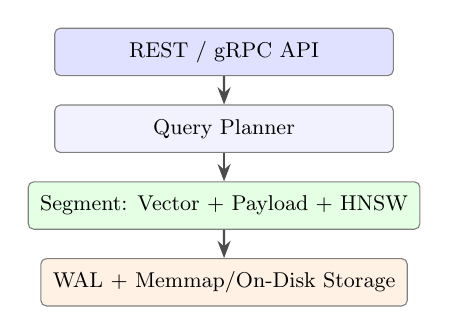
\begin{tikzpicture}[node distance=0.42cm, scale=0.86, transform shape]
    \node[flowbox, fill=blue!12, minimum width=5.0cm] (api) {REST / gRPC API};
    \node[flowbox, below=of api, minimum width=5.0cm] (planner) {Query Planner};
    \node[flowbox, below=of planner, fill=green!10, minimum width=5.0cm] (segment) {Segment: Vector + Payload + HNSW};
    \node[flowbox, below=of segment, fill=orange!10, minimum width=5.0cm] (storage) {WAL + Memmap/On-Disk Storage};
    \draw[flowarrow] (api) -- (planner);
    \draw[flowarrow] (planner) -- (segment);
    \draw[flowarrow] (segment) -- (storage);
\end{tikzpicture}
\caption{Kiến trúc Qdrant xoay quanh segment và payload-aware query path.}
\label{fig:qdrant-arch}
\end{figure}

Kỹ thuật đáng chú ý nhất của Qdrant là tối ưu \textbf{filtered vector search}. Trong RAG production, truy vấn thường kèm điều kiện metadata như tenant, ACL, loại tài liệu hoặc timestamp. Nếu filter được xử lý quá sớm, graph HNSW có thể bị thưa; nếu filter hậu xử lý, Top-K hợp lệ có thể thiếu. Qdrant giải quyết bằng payload index, query planner và filter-aware search path để chọn chiến lược phù hợp theo độ chọn lọc của filter~\cite{qdrantfilter}. Ngoài ra, Qdrant hỗ trợ scalar/product/binary quantization, giúp giảm bộ nhớ hoặc tăng tốc so sánh khi chấp nhận đánh đổi một phần độ chính xác~\cite{jegou2011pq}.

Trade-off của Qdrant là rõ ràng: triển khai gọn, latency thấp và footprint nhỏ trong benchmark của nhóm, nhưng không có BM25 native như Weaviate và không đặt trọng tâm vào kiến trúc phân tán nhiều thành phần như Milvus. Vì vậy Qdrant phù hợp nhất khi bài toán cần filtered retrieval, ít ops và thời gian tích hợp nhanh.

\subsection{Weaviate: hybrid retrieval trong cùng query engine}
\label{sec:weaviate}

Weaviate được thiết kế như một nền tảng vector database \textit{AI-native}. Trong mỗi shard, Weaviate quản lý đồng thời object store, vector HNSW index và inverted index cho BM25/property filtering~\cite{weaviatedocs}. Cách đặt lexical index và vector index cạnh nhau cho phép Weaviate phục vụ native Hybrid Search thay vì phải ghép thêm search engine bên ngoài.

\begin{figure}[H]
\centering
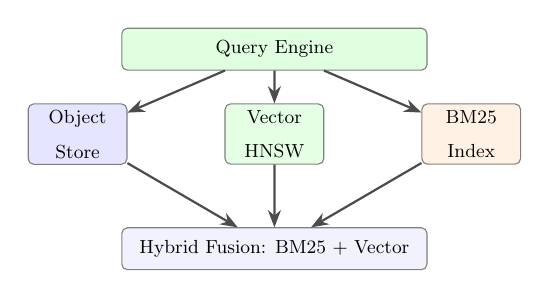
\begin{tikzpicture}[node distance=0.38cm, scale=0.76, transform shape]
    \node[flowbox, fill=green!12, minimum width=5.1cm] (query) {Query Engine};
    \node[flowbox, below left=0.55cm and -0.1cm of query, fill=blue!10, minimum width=1.65cm] (obj) {Object\\Store};
    \node[flowbox, below=0.55cm of query, fill=green!10, minimum width=1.65cm] (hnsw) {Vector\\HNSW};
    \node[flowbox, below right=0.55cm and -0.1cm of query, fill=orange!10, minimum width=1.65cm] (bm25) {BM25\\Index};
    \node[flowbox, below=1.05cm of hnsw, minimum width=5.1cm] (fusion) {Hybrid Fusion: BM25 + Vector};
    \draw[flowarrow] (query) -- (obj);
    \draw[flowarrow] (query) -- (hnsw);
    \draw[flowarrow] (query) -- (bm25);
    \draw[flowarrow] (obj) -- (fusion);
    \draw[flowarrow] (hnsw) -- (fusion);
    \draw[flowarrow] (bm25) -- (fusion);
\end{tikzpicture}
\caption{Weaviate kết hợp object store, HNSW và BM25 trong cùng shard.}
\label{fig:weaviate-arch}
\end{figure}

Hybrid Search hữu ích vì vector search mạnh với paraphrase nhưng có thể bỏ sót mã lỗi, tên riêng hoặc ký hiệu; BM25 lại mạnh với keyword chính xác nhưng không hiểu đồng nghĩa~\cite{robertson2009bm25}. Weaviate dùng tham số $\alpha$ để cân bằng hai tín hiệu và có thể hợp nhất ranking bằng các kỹ thuật như Reciprocal Rank Fusion~\cite{weaviatehybrid,cormack2009rrf}. Hệ module như vectorizer, reranker và generative integration cũng giúp team RAG dựng pipeline nhanh hơn~\cite{weaviatemodules}.

Trade-off của Weaviate là hy sinh một phần độ trễ dense-only để đổi lấy hybrid search và trải nghiệm phát triển thuận tiện hơn. Trong snapshot benchmark của nhóm, Weaviate không nhanh nhất khi chỉ đo dense retrieval, nhưng lợi thế thiết kế của nó nằm ở trường hợp cần keyword evidence và semantic similarity trong cùng API.

\subsection{Milvus: phân tán để phục vụ scale lớn}
\label{sec:milvus}

Milvus chọn kiến trúc \textit{disaggregated}: tách access, coordinator, worker và storage layer~\cite{wang2021milvus,milvusarch}. Proxy nhận request; RootCoord/DataCoord/QueryCoord điều phối metadata, segment và load balancing; DataNode xử lý ingest, QueryNode phục vụ search, IndexNode build index; storage layer dùng object storage, etcd và message queue. Thiết kế này làm deployment phức tạp hơn, nhưng cho phép scale từng vai trò độc lập.

\begin{figure}[H]
\centering
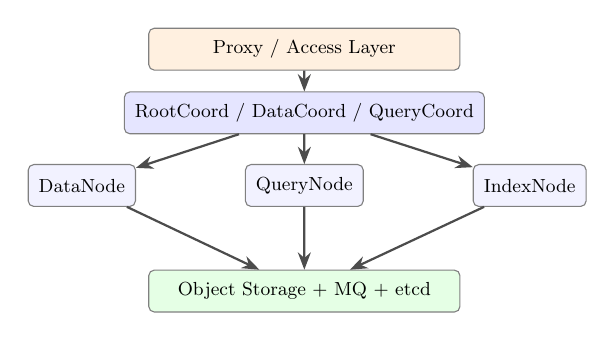
\begin{tikzpicture}[node distance=0.35cm, scale=0.76, transform shape]
    \node[flowbox, fill=orange!12, minimum width=5.2cm] (proxy) {Proxy / Access Layer};
    \node[flowbox, below=of proxy, fill=blue!10, minimum width=5.2cm] (coord) {RootCoord / DataCoord / QueryCoord};
    \node[flowbox, below left=0.5cm and -0.2cm of coord, minimum width=1.65cm] (data) {DataNode};
    \node[flowbox, below=0.5cm of coord, minimum width=1.65cm] (query) {QueryNode};
    \node[flowbox, below right=0.5cm and -0.2cm of coord, minimum width=1.65cm] (index) {IndexNode};
    \node[flowbox, below=1.05cm of query, fill=green!10, minimum width=5.2cm] (storage) {Object Storage + MQ + etcd};
    \draw[flowarrow] (proxy) -- (coord);
    \draw[flowarrow] (coord) -- (data);
    \draw[flowarrow] (coord) -- (query);
    \draw[flowarrow] (coord) -- (index);
    \draw[flowarrow] (data) -- (storage);
    \draw[flowarrow] (query) -- (storage);
    \draw[flowarrow] (index) -- (storage);
\end{tikzpicture}
\caption{Milvus tách compute khỏi storage để scale theo từng vai trò.}
\label{fig:milvus-arch}
\end{figure}

Bên dưới Milvus là \textbf{Knowhere}, lớp trừu tượng bao bọc Faiss, HNSWlib, DiskANN và đường GPU khi có CUDA~\cite{milvusknowheredocs,milvusdiskann,subramanya2019diskann}. Vòng đời dữ liệu cũng cần chú ý khi benchmark: dữ liệu đi qua \texttt{insert}, \texttt{flush}, sealed segment, build index, \texttt{load}, rồi mới search tối ưu~\cite{milvusdocs}. Nếu gộp các bước này vào một metric duy nhất, latency có thể bị diễn giải sai.

Trade-off của Milvus là scale và HA đổi lấy ops complexity. Milvus phù hợp khi corpus lớn, cần replica, GPU hoặc mở rộng từng vai trò; ngược lại, với prototype nhỏ, nhiều dependency như etcd, MinIO và message queue có thể là chi phí vận hành không cần thiết.

\subsection{So sánh kiến trúc}
\label{sec:arch-comparison}

\begin{table}[H]
\centering
\caption{So sánh kiến trúc và trade-off chính.}
\label{tab:arch-compare}
\resizebox{\textwidth}{!}{%
\begin{tabular}{lccc}
\toprule
\textbf{Tiêu chí} & \textbf{Qdrant} & \textbf{Weaviate} & \textbf{Milvus} \\
\midrule
Mô hình & Single binary & Single database service & Distributed services \\
Tối ưu chính & Filtered vector search & Hybrid retrieval & Enterprise scale \\
Index nổi bật & HNSW + payload index & HNSW + BM25 index & Knowhere: Faiss/HNSWlib/DiskANN \\
Keyword/hybrid & Sparse vectors, external logic & BM25 native + vector & Dense/sparse, tùy cấu hình \\
Schema & Payload linh hoạt & Schema/module oriented & FieldSchema chặt \\
Vận hành & Gọn, 1 container & Gọn, nhiều module tùy chọn & Phức tạp hơn, 3+ container \\
Điểm mạnh & Latency/filter/DX & Hybrid RAG ergonomics & HA, GPU, scale per-role \\
Đánh đổi & Ít native lexical search & Dense-only overhead cao hơn & Ops complexity cao \\
\bottomrule
\end{tabular}}
\end{table}

Tóm lại, Qdrant phù hợp khi ràng buộc chính là filtered retrieval và vận hành gọn; Weaviate phù hợp khi cần kết hợp keyword với semantic search; Milvus phù hợp khi scale và HA quan trọng hơn độ đơn giản triển khai.

\section{Đánh giá so sánh}
\label{sec:evaluation}

\subsection{Thiết lập và phương pháp}
\label{sec:experimental-setup}

Nhóm benchmark ba database trong cùng một pipeline để giảm sai lệch do môi trường. Kết quả dưới đây là \textbf{snapshot} trên corpus synthetic 10K chunks và 200 queries; vì vậy nó phù hợp để so sánh trong điều kiện kiểm soát, không phải ranking chung cho mọi workload production.

\begin{table}[H]
\centering
\caption{Cấu hình thực nghiệm và fairness protocol.}
\label{tab:experimental-setup}
\begin{tabular}{lp{9.6cm}}
\toprule
\textbf{Thành phần} & \textbf{Chi tiết} \\
\midrule
Hardware & AMD Ryzen 7 5800H, 16 logical CPUs, 14\,GiB RAM, NVMe SSD 512\,GB \\
Runtime & Arch Linux, Docker Compose v2, Ollama local \\
Embedding / LLM & \texttt{nomic-embed-text} 768 chiều; \texttt{qwen2.5:1.5b} cho RAG chat \\
Index params & HNSW $M=16$, $ef\_construction=128$, $ef\_search=64$, Cosine distance \\
Dataset & 10.000 synthetic chunks, seed = 42; 200 golden queries có tag ground-truth \texttt{[CID:xxxx]} \\
Metrics & Recall@1/5/10, MRR, average latency, recall-latency tradeoff, RAM footprint, DX score \\
\bottomrule
\end{tabular}
\end{table}

Recall@K đo tỷ lệ ground-truth xuất hiện trong top K kết quả, còn MRR đo vị trí trung bình của kết quả đúng:
\[
\text{MRR} = \frac{1}{|Q|}\sum_{i=1}^{|Q|}\frac{1}{\text{rank}_i}.
\]
Toàn bộ tham số HNSW được đọc từ cấu hình chung thay vì hardcode riêng cho từng wrapper, giúp so sánh nhất quán hơn.

\subsection{Kết quả snapshot}

\begin{table}[H]
\centering
\caption{Recall@K, MRR và latency trung bình (corpus = 10K, queries = 200).}
\label{tab:accuracy}
\resizebox{\textwidth}{!}{%
\begin{tabular}{lcccccc}
\toprule
\textbf{Engine} & \textbf{Recall@1} & \textbf{Recall@5} & \textbf{Recall@10} & \textbf{MRR} & \textbf{Avg Latency (ms)} & \textbf{Errors} \\
\midrule
Milvus  & 18.0 & 34.0 & 44.0 & 0.2492 & 4.14 & 0 \\
Qdrant  & 3.0  & 7.5  & 9.5  & 0.0467 & 4.83 & 0 \\
Weaviate & 3.0  & 8.0  & 9.5  & 0.0472 & 14.47 & 0 \\
\bottomrule
\end{tabular}}
\end{table}

Trong snapshot này, Milvus đạt Recall@K và MRR cao nhất, đồng thời giữ average latency thấp. Qdrant và Weaviate có Recall@10 tương đương nhau, nhưng Qdrant nhanh hơn trong dense retrieval. Tuy nhiên, cách đọc đúng không phải là ``Milvus luôn tốt nhất'': benchmark này dùng synthetic corpus, single-node deployment và một bộ tham số index cố định.

Recall tuyệt đối thấp chủ yếu đến từ \textit{vector collapse}. Corpus synthetic được sinh từ số lượng template ít; nhiều chunk gần như đồng nghĩa nên embedding model gom chúng vào cùng vùng không gian. Khi đó database có thể tìm đúng cụm ngữ nghĩa nhưng chưa chắc trả đúng ID ground-truth cụ thể. Đây là giới hạn của dataset benchmark, không phải bằng chứng rằng các database có chất lượng retrieval thấp trong mọi corpus thật.

\subsection{Recall-latency tradeoff và filter}

\begin{table}[H]
\centering
\caption{Tradeoff sweep: Recall (\%) / Avg latency (ms) theo top\_k.}
\label{tab:tradeoff}
\resizebox{\textwidth}{!}{%
\begin{tabular}{lcccccc}
\toprule
\textbf{Engine} & \textbf{K=1} & \textbf{K=2} & \textbf{K=5} & \textbf{K=10} & \textbf{K=20} & \textbf{K=50} \\
\midrule
Milvus  & 18.0 / 3.65 & 24.0 / 3.68 & 34.0 / 3.67 & 44.0 / 3.88 & 62.0 / 3.85 & 80.0 / 4.17 \\
Qdrant  & 3.0 / 4.57 & 3.5 / 4.71 & 7.5 / 4.80 & 9.5 / 4.87 & 17.5 / 5.10 & 27.0 / 5.82 \\
Weaviate & 3.0 / 16.19 & 3.5 / 15.77 & 8.0 / 15.39 & 9.5 / 15.49 & 15.5 / 14.96 & 24.5 / 15.66 \\
\bottomrule
\end{tabular}}
\end{table}

Milvus giữ đường tradeoff tốt nhất trên snapshot này: Recall tăng đến 80\% ở K=50 trong khi latency vẫn quanh 4\,ms. Qdrant có latency tăng chậm khi K tăng, cho thấy chi phí biên để lấy thêm kết quả khá nhỏ. Weaviate có latency ổn định quanh 15--16\,ms; kết quả này phản ánh dense retrieval path trong benchmark, chưa thể hiện đầy đủ lợi thế native hybrid search của Weaviate.

Qdrant được đo riêng với filter metadata sau warmup: dense-only baseline đạt 3.97\,ms; equality filter đạt 5.29\,ms; range filter đạt 5.20\,ms; combined filter đạt 5.73\,ms. Overhead +1.2--1.8\,ms cho thấy trong thí nghiệm này payload filter tạo chi phí nhỏ và vẫn phù hợp với RAG cần tenant/ACL filtering.

\subsection{Tài nguyên và Developer Experience}

\begin{table}[H]
\centering
\caption{Tài nguyên và DX trong codebase benchmark của nhóm.}
\label{tab:dx-resource}
\resizebox{\textwidth}{!}{%
\begin{tabular}{lccc}
\toprule
\textbf{Metric} & \textbf{Qdrant} & \textbf{Weaviate} & \textbf{Milvus} \\
\midrule
RAM sau benchmark & $\sim$178\,MB & $\sim$200--300\,MB & $\sim$398\,MB \\
Containers cần thiết & 1 & 1 & 3+ \\
SLOC wrapper & \textbf{232} & 306 & 379 \\
Cyclomatic complexity & \textbf{24} & 59 & 36 \\
Third-party imports & \textbf{2} & 4 & 3 \\
Composite DX score (thấp hơn tốt hơn) & \textbf{190.0} & 307.0 & 290.5 \\
\bottomrule
\end{tabular}}
\end{table}

Qdrant có footprint và DX score tốt nhất trong codebase của nhóm, phù hợp với prototype hoặc team nhỏ. Milvus dùng nhiều tài nguyên và dependency hơn, nhưng đó là chi phí đi kèm kiến trúc phân tán. Weaviate nằm giữa hai cực: triển khai vẫn gọn, nhưng wrapper phức tạp hơn vì schema, module và hybrid query surface.

\subsection{Hạn chế}

Thí nghiệm có bốn giới hạn chính. Thứ nhất, synthetic corpus gây vector collapse nên recall tuyệt đối không đại diện cho tài liệu thật. Thứ hai, benchmark chạy single-node nên chưa đo được lợi thế phân tán của Milvus. Thứ ba, Docker resource limits và warmup/cache có thể ảnh hưởng latency tail. Thứ tư, Weaviate được đánh giá chủ yếu bằng dense retrieval snapshot, trong khi điểm mạnh thiết kế của nó là hybrid retrieval. Vì vậy, kết quả nên được đọc như bằng chứng cho một workload cụ thể, không phải kết luận vĩnh viễn.

\section{Thảo luận}
\label{sec:discussion}

Kết quả kiến trúc và benchmark cho thấy lựa chọn Vector Database nên bắt đầu từ ràng buộc hệ thống thay vì từ một bảng xếp hạng tuyệt đối. Ba công cụ đều có thể dùng cho RAG, nhưng mỗi công cụ tối ưu cho một điểm khác nhau: Qdrant cho filtered retrieval gọn nhẹ, Weaviate cho hybrid search, Milvus cho scale và HA.

\begin{table}[H]
\centering
\caption{Ma trận quyết định theo use case.}
\label{tab:decision-matrix}
\begin{tabularx}{\textwidth}{p{3.6cm}X}
\toprule
\textbf{Use case} & \textbf{Khuyến nghị} \\
\midrule
Prototype / POC nhanh & Qdrant, vì triển khai 1 container, wrapper ít dòng code và DX score thấp nhất trong codebase nhóm. \\
RAG cần keyword + semantic & Weaviate, vì native hybrid search kết hợp BM25 và vector trong cùng query surface~\cite{weaviatehybrid}. \\
Enterprise hoặc corpus rất lớn & Milvus, vì kiến trúc disaggregated hỗ trợ scale per-role, HA và Knowhere/GPU/DiskANN~\cite{milvusarch}. \\
Multi-tenant, ACL, filter-heavy RAG & Qdrant, vì payload-oriented design và filter-aware search path phù hợp metadata filtering. \\
Team nhỏ, ít kinh nghiệm vận hành & Qdrant hoặc Weaviate; Milvus chỉ nên chọn khi nhu cầu scale đủ lớn để bù chi phí ops. \\
\bottomrule
\end{tabularx}
\end{table}

Nếu ưu tiên latency và vận hành gọn, Qdrant là lựa chọn dễ bắt đầu nhất. Nếu chất lượng retrieval phụ thuộc cả từ khóa chính xác lẫn ngữ nghĩa, Weaviate có lợi thế thiết kế dù dense-only benchmark không phải điểm mạnh nhất của nó. Nếu bài toán cần corpus rất lớn, replica, GPU hoặc tách riêng ingest/search/indexing, Milvus có kiến trúc phù hợp hơn, nhưng yêu cầu đội vận hành hiểu Docker/Kubernetes và các dependency như object storage, etcd, message queue.

Với Qdrant, điểm mạnh không chỉ nằm ở thời gian truy vấn trong snapshot mà còn ở đường cong vận hành. Mô hình collection/point/payload dễ ánh xạ sang ứng dụng RAG thông thường: mỗi chunk có embedding, metadata và nội dung tham chiếu. Khi hệ thống cần lọc theo tenant, nguồn dữ liệu, vai trò người dùng hoặc thời gian cập nhật, payload index giúp giảm phần không gian tìm kiếm trước hoặc trong quá trình truy vấn tùy kế hoạch thực thi. Trong nhóm ba công cụ, Qdrant vì vậy là lựa chọn hợp lý khi team muốn đi từ prototype lên production nhỏ-vừa mà chưa muốn gánh nhiều service phụ trợ. Trade-off là khi yêu cầu scale ngang phức tạp, nhiều pipeline ingest song song hoặc HA nghiêm ngặt, Qdrant cần được thiết kế cụm cẩn thận hơn thay vì chỉ dựa vào cấu hình single-node.

Với Weaviate, cần đọc benchmark dense-only một cách công bằng. Nếu chỉ đo vector search trên cùng embedding, Weaviate có thể không luôn dẫn đầu về latency hoặc footprint; tuy nhiên đó chưa phải workload đại diện nhất cho công cụ này. Weaviate mạnh khi truy vấn gồm cả ngữ nghĩa và từ khóa: ví dụ tài liệu pháp lý có số điều khoản, catalog có mã sản phẩm, ticket hỗ trợ có tên lỗi hoặc log code. Trong các trường hợp này, BM25/inverted index và vector HNSW bổ sung cho nhau, còn hybrid score giúp hệ thống tránh bỏ sót kết quả chứa token chính xác nhưng embedding không đủ gần. Vì vậy, Weaviate phù hợp với đội phát triển muốn một API retrieval giàu tính năng hơn là một ANN service tối giản.

Với Milvus, lợi thế xuất hiện rõ hơn khi corpus và tổ chức vận hành đủ lớn. Kiến trúc tách Proxy, Coordinator, QueryNode, DataNode và IndexNode cho phép scale từng vai trò theo bottleneck: nhiều truy vấn thì tăng QueryNode, ingest nặng thì chú ý DataNode và message queue, build index lớn thì tăng IndexNode hoặc cân nhắc GPU. Đây là kiểu thiết kế quen thuộc trong Big Data system: đổi sự đơn giản của single binary lấy khả năng mở rộng, cô lập lỗi và tối ưu theo workload. Do đó, kết luận ``Milvus đạt Recall@K cao nhất trong snapshot'' nên được hiểu là tín hiệu về năng lực index/search, không đồng nghĩa Milvus luôn là lựa chọn tốt nhất cho mọi team.

Một cách đọc thực dụng hơn là xem benchmark như bài kiểm tra điều kiện. Snapshot 10K synthetic chunks và 200 queries giúp so sánh hành vi tương đối trong môi trường kiểm soát, nhưng chưa bao phủ dữ liệu đa miền, update/delete liên tục, phân quyền phức tạp, warm-up cache dài hạn hoặc failure recovery. Khi áp dụng vào dự án thật, nhóm nên tái chạy quy trình đánh giá trên dữ liệu nội bộ, giữ nguyên ba nhóm chỉ số: chất lượng truy hồi, chi phí tài nguyên và độ phức tạp vận hành. Lựa chọn tốt nhất không phải công cụ thắng nhiều cột nhất, mà là công cụ có điểm mạnh trùng với ràng buộc quan trọng nhất của hệ thống.

Xu hướng chung của Vector Database là tiến tới retrieval đa tín hiệu: dense vector, sparse/keyword, metadata filter, reranking và multi-modal embedding. Vì vậy, benchmark trong báo cáo nên được xem là quy trình đánh giá có thể lặp lại, không phải kết luận cuối cùng cho mọi phiên bản và workload.

\section{Kết luận}
\label{sec:conclusion}

Báo cáo đã phân tích Qdrant, Weaviate và Milvus từ bốn góc nhìn: mục tiêu thiết kế, trạng thái mã nguồn mở/chi phí, kiến trúc nội bộ và kết quả benchmark trong hệ thống RAG của nhóm. Cả ba đều là lựa chọn nghiêm túc cho vector search, nhưng chúng tối ưu cho ba ràng buộc khác nhau.

Trong snapshot 10K synthetic chunks, Milvus đạt Recall@K cao nhất; Qdrant nổi bật ở footprint, latency filter và DX; Weaviate nổi bật ở native hybrid retrieval. Do đó, kết luận quan trọng không phải là chọn một ``winner'' tuyệt đối, mà là chọn công cụ theo use case: Qdrant cho filtered RAG gọn nhẹ, Weaviate cho keyword + semantic retrieval, và Milvus cho scale/HA.

Đóng góp chính của nhóm là xây dựng một quy trình đánh giá có thể lặp lại: cùng corpus, cùng query, cùng tham số index, cùng pipeline và cùng dashboard trực quan hóa. Đây là cách tiếp cận thực tế hơn so với việc so sánh công cụ chỉ bằng mô tả marketing hoặc một metric đơn lẻ.


% References
\input{ref/ref.tex}
\end{document}
